\chapter{OOP 2: Datenkapselung}
\renewcommand{\chaptertitle}{OOP 2: Datenkapselung}

\lehead[]{\normalfont\sffamily\hspace*{-2.00cm}\textcolor{white}{\colorbox{lightblue}{\makebox[1.60cm][r]{\thechapter}}}\hspace{0.17cm}\textcolor{lightblue}{\chaptertitle}}
\rohead[]{\textcolor{lightblue}{\chaptertitle}\normalfont\sffamily\hspace*{0.17cm}\textcolor{white}{\colorbox{lightblue}{\makebox[1.60cm][l]{\thechapter}}}\hspace{-2.00cm}}
%\chead[]{}
\rehead[]{\textcolor{lightblue}{AvHG, Inf, My}}
\lohead[]{\textcolor{lightblue}{AvHG, Inf, My}}

\lstset{style=myJava}

\section{Problembeschreibung}

Gegeben ist eine Klasse \myClass{Tisch} mit folgendem Code:

\begin{lstlisting}
import java.awt.*;

public class Tisch {
  private int x, y;        æ// linke obere Ecke
æ  public int hoehe = 50;
  public int breite = 100; æ// Wichtig: Die Breite muss immer das Doppelte der Höhe sein!
æ
  public Tisch(int x, int y) {
    this.x = x;
    this.y = y;
  }
  
  public void zeichnen(Graphics g) {
    g.fillRect(x, y, breite, 10);
    g.fillRect(x + 5, y, 10, hoehe);
    g.fillRect(x + breite - 15, y, 10, hoehe);
  }
}
\end{lstlisting}

Für alle Tische des Herstellers „Fantastika“ besteht die Vorgabe, dass die
Breite immer das Doppelte der Höhe betragen muss. Ein unachtsamer
Programmierer, der die Aufgabe hatte, für die Anwendung eine hübsche
Bedienungsoberfläche zu schreiben, hat diese Vorgabe jedoch nicht beachtet. Die
Bedienungsoberfläche bietet dem Benutzer die Möglichkeit, die Höhe des Tisches
unabhängig von der Breite zu ändern:

\begin{center}
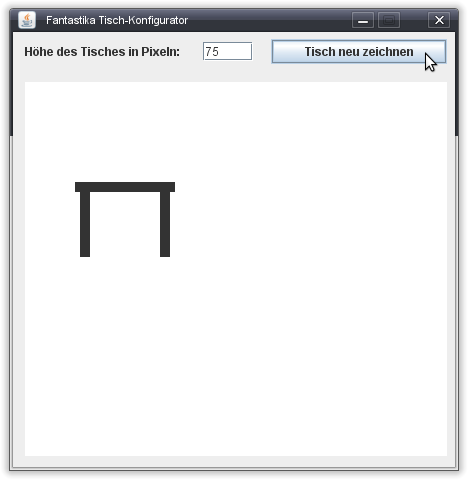
\includegraphics[width=0.6\textwidth]{./inf/SEKII/11_Java_Datenkapselung/tisch-konfigurator.png}
\end{center}

Die Höhe wird von außen nach Eingabe des Benutzers z.B.\ mit folgender Anweisung
geändert:

\begin{lstlisting}
tisch1.hoehe = 100;      æ// tisch1 ist ein Objekt der Klasse Tisch
\end{lstlisting}

Natürlich wird jetzt ordentlich gemeckert und der Programmierer muss die
Oberfläche umschreiben. Aber es wäre ja viel schöner gewesen, wenn diese
Fehlbenutzung von vornherein durch geschickte Programmierung verhindert worden
wäre.

\textbf{Wie kann man innerhalb der Klasse \myClass{Tisch} dafür sorgen, dass
die Anforderung „die Breite ist das Doppelte der Höhe“ nicht verletzt werden kann,
auch wenn der ahnungslose Benutzer der Klasse ausschließlich die Höhe
verstellt?}


\section{Lösung: Datenkapselung}

Wenn mehrere Programmierer zusammen ein großes Programm schreiben,
müssen sie sich sorgfältig absprechen, damit die einzelnen Programmteile
korrekt zusammenarbeiten. Jeder Programmierer entwirft für seine
Programmteile eine sogenannte \emph{öffentliche Methodenschnittstelle}. Diese Schnittstelle besteht
aus den öffentlichen (\lstinline|public|) Methoden einer Klasse,
die andere Programmierer benutzen können. Eine Schnittstelle sollte möglichst
übersichtlich und für andere leicht verständlich sein. Bewährt hat sich dabei
das Prinzip der \emph{Datenkapselung}:

\textbf{Datenkapselung} hat zwei Aspekte:

\begin{compactenum}
\item Die bereits im Kapitel \ref{ch:KlassenUndObjekte} beschriebene
Verknüpfung von Daten und Methoden: In einer Klasse werden zum einen die Daten
selbst als Attribute der Klasse definiert. Zum anderen werden in der Klasse auch
alle Operatoren (Methoden) definiert, die auf Objekte dieser Klasse anzuwenden
sind.
\item Das sogenannte \emph{Geheimnisprinzip}: Alle Attribute einer Klasse
(also alle ihre Daten) werden vor dem direkten Zugriff von außen versteckt (d.\,h.\ sie
sind \lstinline|private|). Andere Programmierer können die Objekte der Klasse
nur über eine Reihe sorgfältig definierter Methoden auslesen oder verändern. 
In der Fachsprache nennt man Methoden zum Auslesen eines Attributs \emph{Getter} 
(z.\,B.\ \lstinline|getHoehe()|) und Methoden zum Verändern eines Attributs \emph{Setter} 
(z.\,B.\ \lstinline|setHoehe(int neueHoehe)|).

Auf diese Weise wird sichergestellt, dass die Benutzer der Klasse nicht versehentlich oder
absichtlich die Funktionalität der Klasse unterwandern. In den öffentlichen
Setter-Methoden der Klasse wird geprüft, dass die Variablen keine verbotenen
Werte (wie z.B.\ negative Längen) annehmen können. Außerdem wird darauf geachtet, dass 
alle notwendigen Anpassungen anderer Attribute (Seiteneffekte) automatisch mit ausgeführt werden.
\end{compactenum}

Für unsere Klasse \myClass{Tisch} sieht die gekapselte Lösung daher so aus:

\begin{lstlisting}
public class Tisch {
  private int x, y;         æ// Alle Attribute sind private!
æ  private int hoehe = 50;
  private int breite = 100;

  public Tisch(int x, int y) {
    this.x = x;
    this.y = y;
  }

  public int getHoehe() {   æ// Getter-Methode zum Auslesen
æ    return hoehe;
  }

  public void setHoehe(int neueHoehe) { æ// Setter-Methode mit Konsistenzprüfung
æ    if (neueHoehe > 0) {
      this.hoehe = neueHoehe;
      this.breite = 2 * neueHoehe;      æ// Breite wird automatisch angepasst!
æ    }
  }
  ...
}
\end{lstlisting}

Neben der \textbf{Sicherstellung der korrekten Arbeitsweise} der Klasse bietet
die Datenkapselung noch weitere Vorteile:

\begin{compactitem}
\item[\textbf{Benutzbarkeit:}] Die Schnittstelle ist für andere Programmierer
übersichtlich. Sie brauchen sich nicht mit der internen Arbeitsweise der Klasse
auseinanderzusetzen (Black-Box-Prinzip).
\item[\textbf{Wartbarkeit:}] Wenn die interne Funktionalität der Klasse
verändert wird, braucht der Code, in dem die Klasse verwendet wird, nicht
ebenfalls umgeschrieben zu werden, sofern die Methodenschnittstelle unverändert bleibt.
Änderungen und Erweiterungen der Klasse sind dadurch problemlos möglich.
\end{compactitem}
